\documentclass[12pt, letterpaper]{article}
\usepackage[utf8]{inputenc}
\usepackage{graphicx}
\graphicspath{ {./images/} }
\usepackage{wrapfig}
\usepackage[left=2cm, right=2cm, top=2.5cm]{geometry}
\usepackage{indentfirst}
\usepackage{caption}
\usepackage{subcaption}
\usepackage{amsmath}
\usepackage{sidecap}
\usepackage{hyperref}
\usepackage{tikz}
\usepackage{physics}
\usepackage{fancyhdr}
\usepackage{setspace}
\usepackage[font=footnotesize]{caption}


\title{A more precise measurement of $D$ meson mass difference through $D^{+}_{(s)} \rightarrow K^{+}K^{-}\pi^{+}$ decay\vspace{5mm}}

\author{\vspace{3mm} \textbf{John Bodenschatz}\\
	\vspace{3mm}
  \textit{Physics Capstone}\\
  University of Cincinnati\\}
  
\date{\vspace{5mm} April 26, 2021}

\setlength\parindent{24pt}



\pagestyle{fancy}
\pagestyle{fancy}
\fancyhf{}
\rhead{Bodenschatz}
\lhead{University of Cincinnati}
\lfoot{Physics Capstone}
\rfoot{LHCB Preliminary \quad \thepage}



\begin{document}

\maketitle

\begin{center}
\textbf{Abstract}
\end{center}
Using the three body decay of $D^{+}_{(s)} \rightarrow K^{+}K^{-}\pi^{+}$, we improve the statistical error of the mass difference measurement $m_{D^+_s} - m_{D^+}$. The most recent high precision measurement (2013) is $98.68 \pm 0.03\text{(stat)} \pm 0.04\text{(syst)}$ MeV/$c^2$ \cite{lhcb}. From 2017 LHCb data, we yield $4,970,691 \pm 11,548$ $D^+$ signal events and $8,524,400 \pm 17,505$ $D^+_s$ signal events. We measure $98.900 \pm 0.0036\text{(stat)} \pm x.xxx\text{(syst)}$ MeV/$c^2$. Through future work we will be able to establish a systematic uncertainty on the same order as statistical.







\begin{tikzpicture}[remember picture,overlay]
    \node[xshift=-7.0cm,yshift=3.5cm] at (current page.south){
\includegraphics[width=.2\linewidth]{lhcb_logo.jpg}};
        \node[xshift=-0.1cm,yshift=4.2cm] at (current page.south){
\includegraphics[width=.23\linewidth]{UC_ID_PrimaryBlackRed.pdf}};
        \node[xshift=7.0cm,yshift=3.5cm] at (current page.south){
\includegraphics[width=.23\linewidth]{nsflogo.png}};
\end{tikzpicture}




\newpage
\section*{Social Responsibility Statement}
\begin{minipage}{0.9\textwidth}
    \baselineskip=2\baselineskip
Throughout the past year I have had the pleasure of studying high energy physics and learning all about CERN, LHCb, and more thanks to Dr. Michael Sokoloff. I have been able to work on CERN's global computing system to acquire vast amounts of data to make a real physics measurement. I have also learned a great deal along the way about the research process and how I work best when faced with problems. As for the project itself, these sort of studies are conducted fairly frequently and for a good reason. Making more and more high precision measurements is a pinnacle of experimental physics. Every significant digit matters and can have an impact on how we understand the results, especially on the scale of mesons and other such particles. I have vastly developed my skills as an individual and collaborative researcher during this time. At the beginning of my time with Dr. Sokoloff, there were three things he said he wanted us to learn: how to communicate effectively, how to work with others, and how to think critically about certain problems. I have worked a great dealing at developing my ability to accomplish these three tasks, for both research and life. The opportunities provided to me through this research will forever have an impact on my future endeavors. Following graduation, I will be attending Marquette University where I will pursue a Ph.D. in Computational Mathematical and Statistical Sciences. I am hoping to develop a deeper understanding of the application of computational techniques and how they can solve real-world problems. My education in physics has outfitted me with an incredible set of analytical tools that will certainly go far in life.


\end{minipage}








\newpage
\section{Introduction}
Mesons are a family of colorless subatomic particles composed of quark-antiquark pairs. They are particularly sensitive to the strong force, the force responsible for holding together atomic nuclei and governing interactions between particles containing quarks. By studying the mass difference of mesons, we can determine constants such as $m_c / m_b$ which are fundamental parameters of Quantum Chromodynamics (QCD) \cite{theory}. QCD, analogous to Quantum Electrodynamics (QED), involves the theory describing the action of the strong force \cite{QCD}. For this study in particular, the mesons are composed of the following constituent quarks:

\begin{center}
$\ket{D^+} = \ket{c\bar{d}}$ \\
$\ket{D^+_s} = \ket{c\bar{s}}$ 
\end{center}

These mesons will be used to measure the mass difference $m_{D^+_s} - m_{D^+}$. The most recent high precision measurement of this mass difference was done on Run 1 data from the LHCb experiment \cite{lhcb}. This study yielded $68,787 \pm 321 $ $D^+$ events and $284,694 \pm 540 $ $D^+_s$ events and resulted in a measurement of $m_{D^+_s} - m_{D^+} = 98.68 \pm 0.03 \pm 0.04$ MeV. The Particle Data Group (PDG) average for this measurement is currently listed as $98.69 \pm 0.05$ MeV \cite{pdg}.

By an early estimate of the amount of data in Run 2 compared to Run 1 at the LHC, we estimate that it may be possible to reduce the statistical error of this measurement by a factor of 10. In 2017 alone, 40 PB of data produced from LHC experiments were recorded at the CERN data center \cite{cerncomp}.




\begin{figure}[h!]
\centering
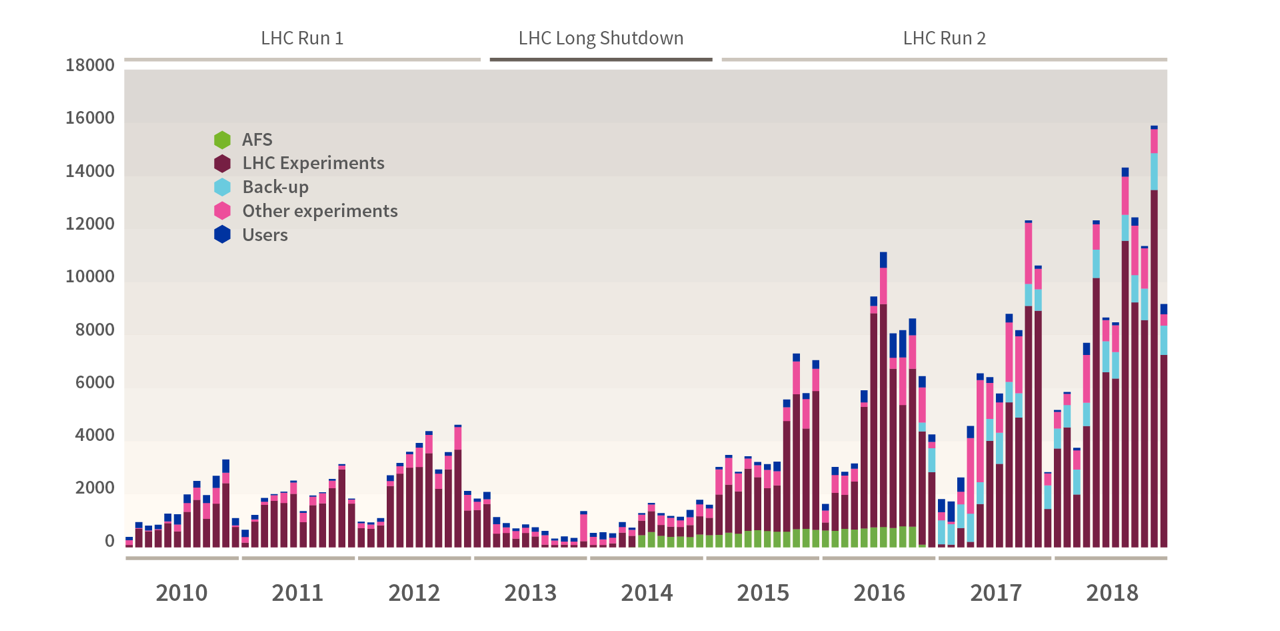
\includegraphics[width=0.83\linewidth]{lhc_data.png}
\caption{Image from CERN Computing showing the data (TB) recorded at CERN month-by-month.}
\label{fig:storage}
\end{figure}







\newpage
\section{Detector and Dataset}
The LHCb detector is part of one of four main experiments at CERN’s Large Hadron
Collider (LHC) in Geneva, Switzerland. This experiment's focus is to study the slight differences between matter and anti-matter by studying particles containing b quarks.  As depicted in Figure \ref{fig:detector}, the 5600-ton detector is composed of many sub-detectors that span 10 meters tall, 13 meters wide, and 20 meters along the beam pipe \cite{detector2}. Unlike some other detectors at the LHC, the LHCb experiment is built to measure forward particles- or particles that are projected in one direction roughly along the beam pipe. 

\begin{figure}[h!]
\centering
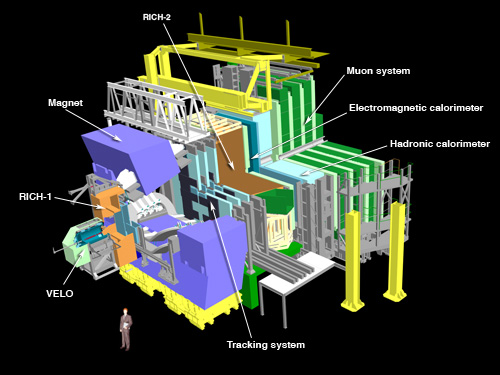
\includegraphics[width=0.6\linewidth]{detector.jpg}
\caption{Diagram of the LHCb detector pointing out several useful sub-detectors.}
\label{fig:detector}
\end{figure}

A system of ring-imaging Cherenkov detectors (RICH1 and RICH2) are used to identify charged hadrons that pass through the detector. The two mesons that compose the daughters of the studied decay, the kaon and the pion,  are both hadronic. The magnet on the detector is used to bend charged particles slightly away from the beam and into other parts of the sub-detectors, namely the tracking system. The tracking system is composed of three stations of silicon-strip detectors and straw drift tubes (sometimes referred to as T-Stations). The T-Stations are used to measure the momentum of particles passing through.

When operational, the LHCb records approximately 10 million collisions per
second \cite{events}. After filtering, only about 1 million events are saved to storage; this translates to 35 GB of data per second. The detector observes and records decay channels from many particles. For this analysis we are only interested in the $D^{+}_{(s)} \rightarrow K^{+}K^{-}\pi^{+}$ decay mode. Data for this analysis was taking from all 2017 (Run 2) proton-proton collisions, totaling to 1.3 TB of data before cuts. The flow of data as taken from the detector to analysis can be seen in Figure \ref{fig:dataflow}, outlined in red.
 



\begin{figure}[h!]
\centering
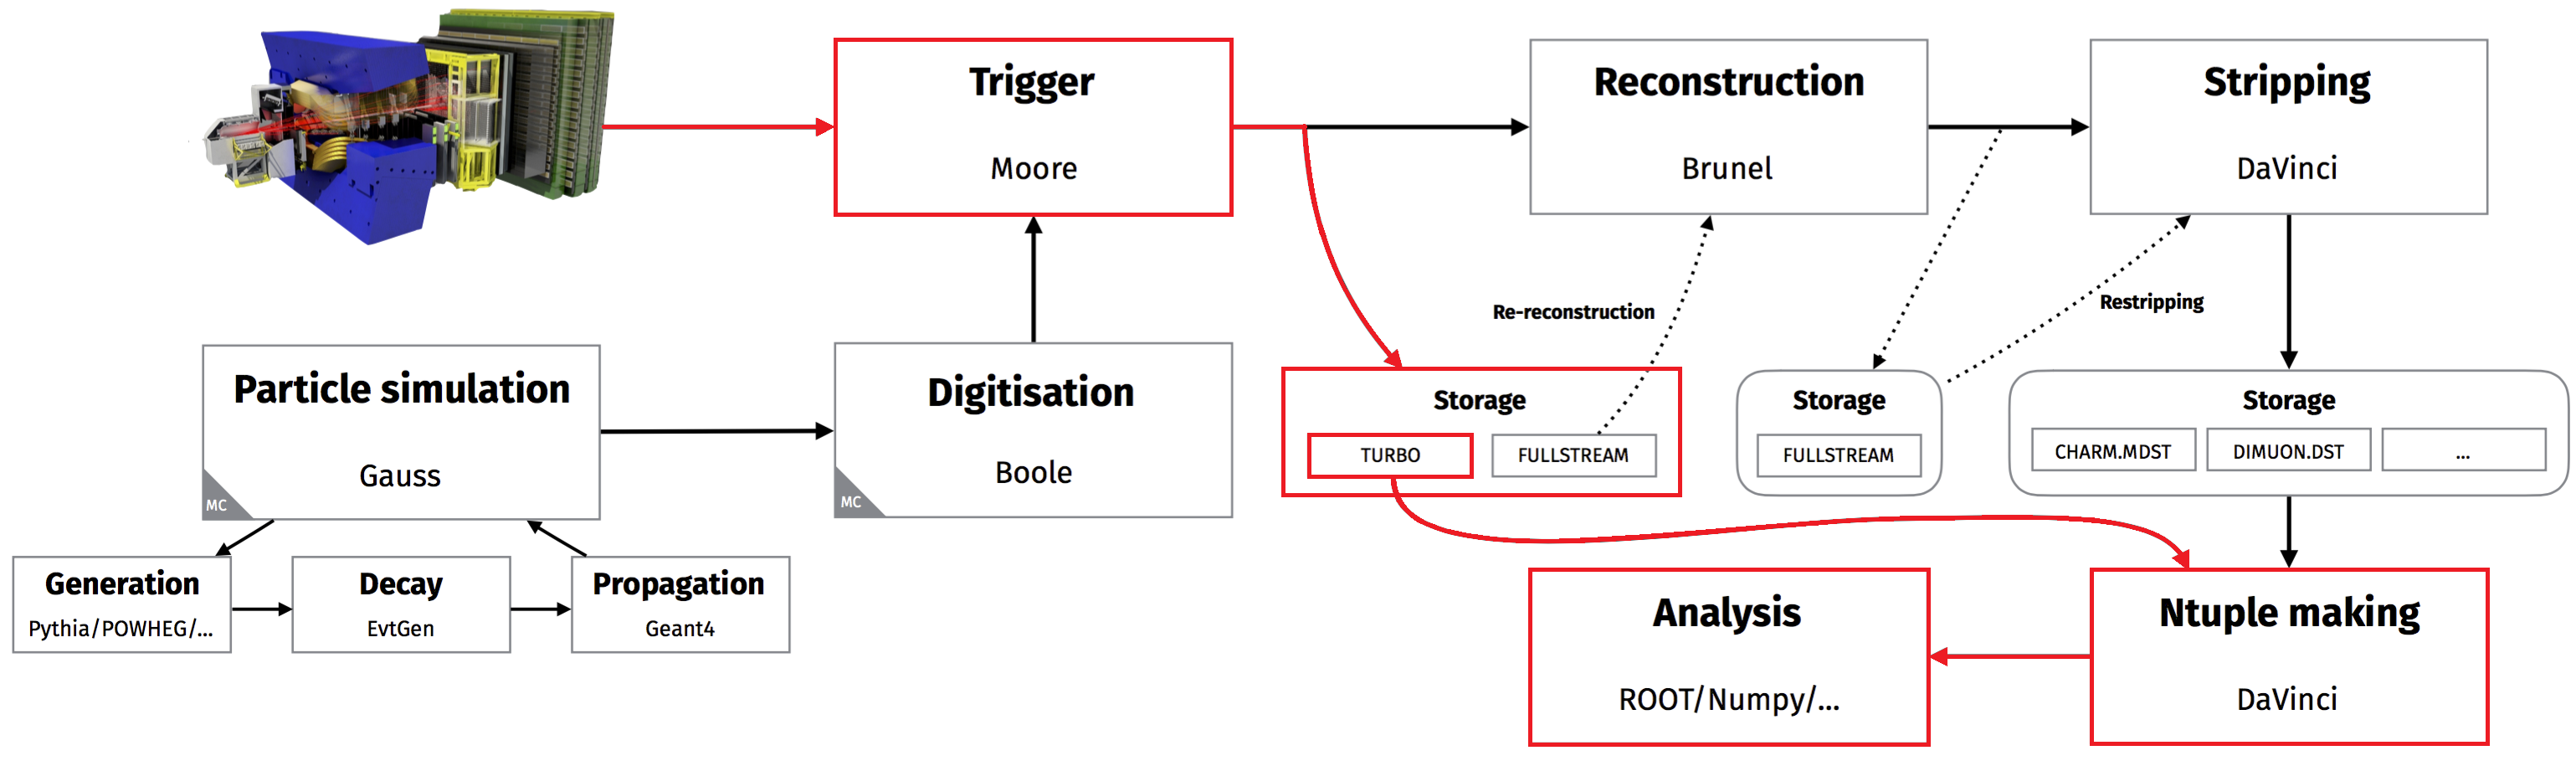
\includegraphics[width=1\linewidth]{lhcb_run_2_data_flow.png}
\caption{Red path highlighting the flow of data used for this study.}
\label{fig:dataflow}
\end{figure}







\section{Selection}
Not all raw data that is collected is used for the analysis. Each candidate event must pass a set of selection criteria, often referred to as "cuts", to be accepted for fitting. The goal in cutting on the data is to reduce the background while retaining a large amount of signal events, i.e., increasing the signal-to-background ratio. However, cuts must also remain physically valid and justifiable. We cannot cut on a variable simply because it gives us a better result- we must be able to say what purpose the cut serves with regards to eliminating "bad" events.

The raw data provided us with $3.5 \cdot 10^8$ $D^+$ candidate events and $5.0 \cdot 10^8$ $D^+_s$ candidate events. Figure \ref{fig:precut} shows a sample of the raw $D^+$ data before any cuts are applied. Here, the signal-to-background ratio is about 8. 

\begin{figure}[h!]
\centering
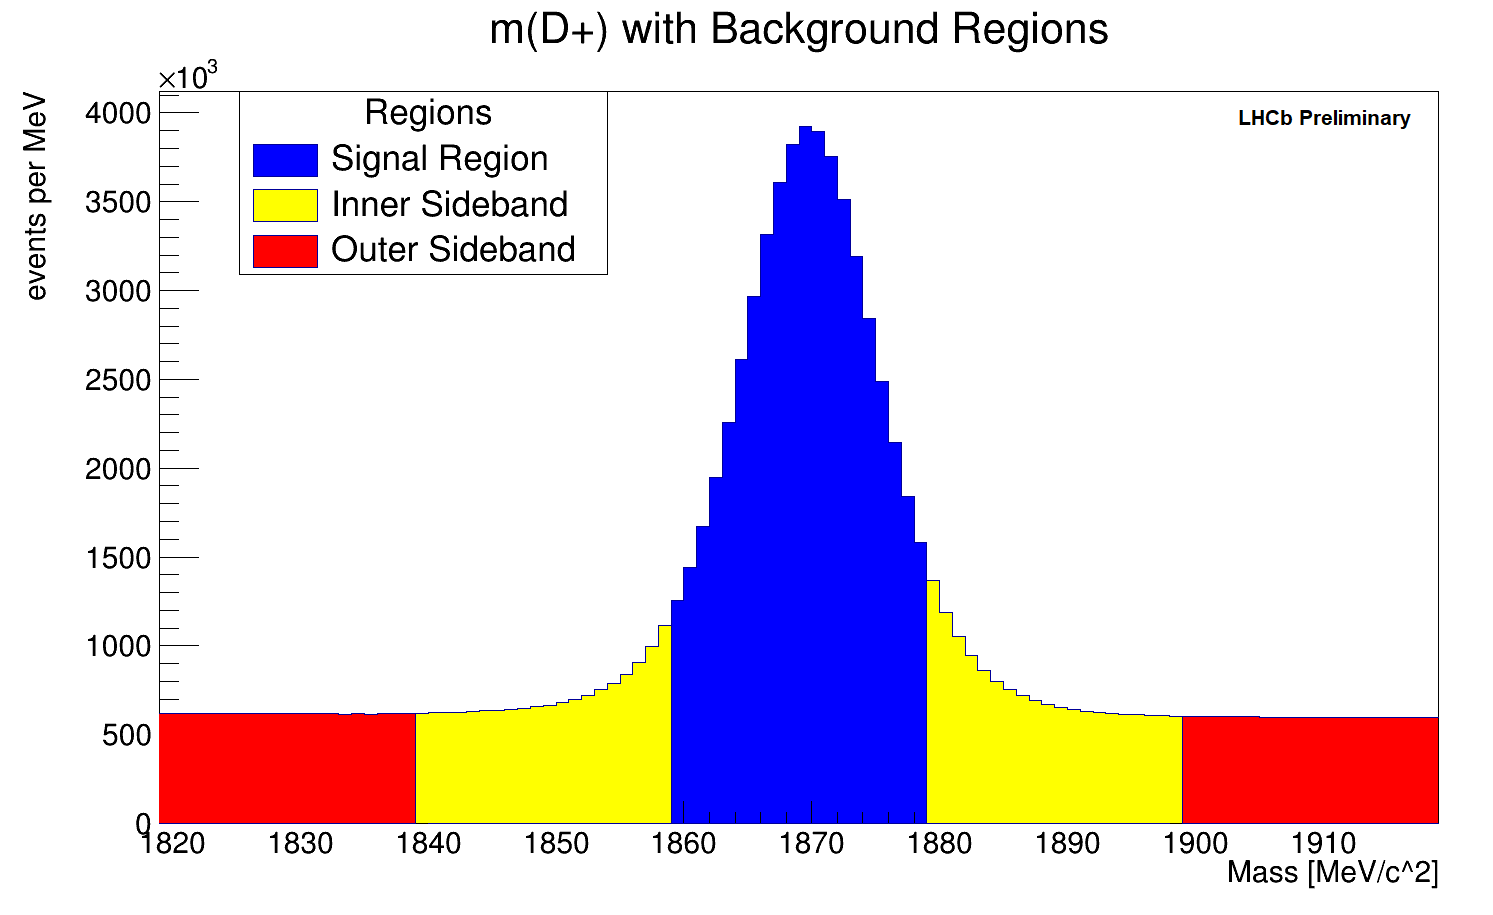
\includegraphics[width=0.7\linewidth]{dp_mdp.png}
\caption{Sample of the $D^+$ data before cuts are applied.}
\label{fig:precut}
\end{figure}

\newpage
To select well-identified kaons (pions) the difference in the logarithms of the global likelihood of the kaon (pion) hypothesis relative to the pion (kaon) hypothesis provided by the ring-imaging Cherenkov detectors is required to be greater than five (zero) \cite{lhcb}. In addition to this, the product of the neural net likelihoods of the kaon hypothesis for each kaon and the pion hypothesis for the pion is constrained to be greater than 0.7. These cuts, in effect, ensure that the kaons and pions as identified by the detector truly \textit{are} kaons and pions, rather than some other misidentified charged hadron.

To eliminate kinematic reflections due to misidentified pions, the invariant mass of at least one kaon pair is required to be within $±10$ MeV/$c^2$ of the nominal value of the $\phi$ meson mass \cite{lhcb, kinematics}. This means that the D meson decay for our study will be dominated by those including an intermediate $\phi$ meson. This cut can be seen illustrated in Figure \ref{fig:dalitz}, a Dalitz plot showing the phase-space of the $D^+$ mother particle. The vertical band in the right figure is the so-called $\phi$ region. By selecting only these decays, we are able to reduce a significant amount of background from the mass-fitting; almost all of the events in the background of the Dalitz plot are cut. 


\begin{figure}[h!]
\centering
\begin{subfigure}{.5\textwidth}
  \centering
  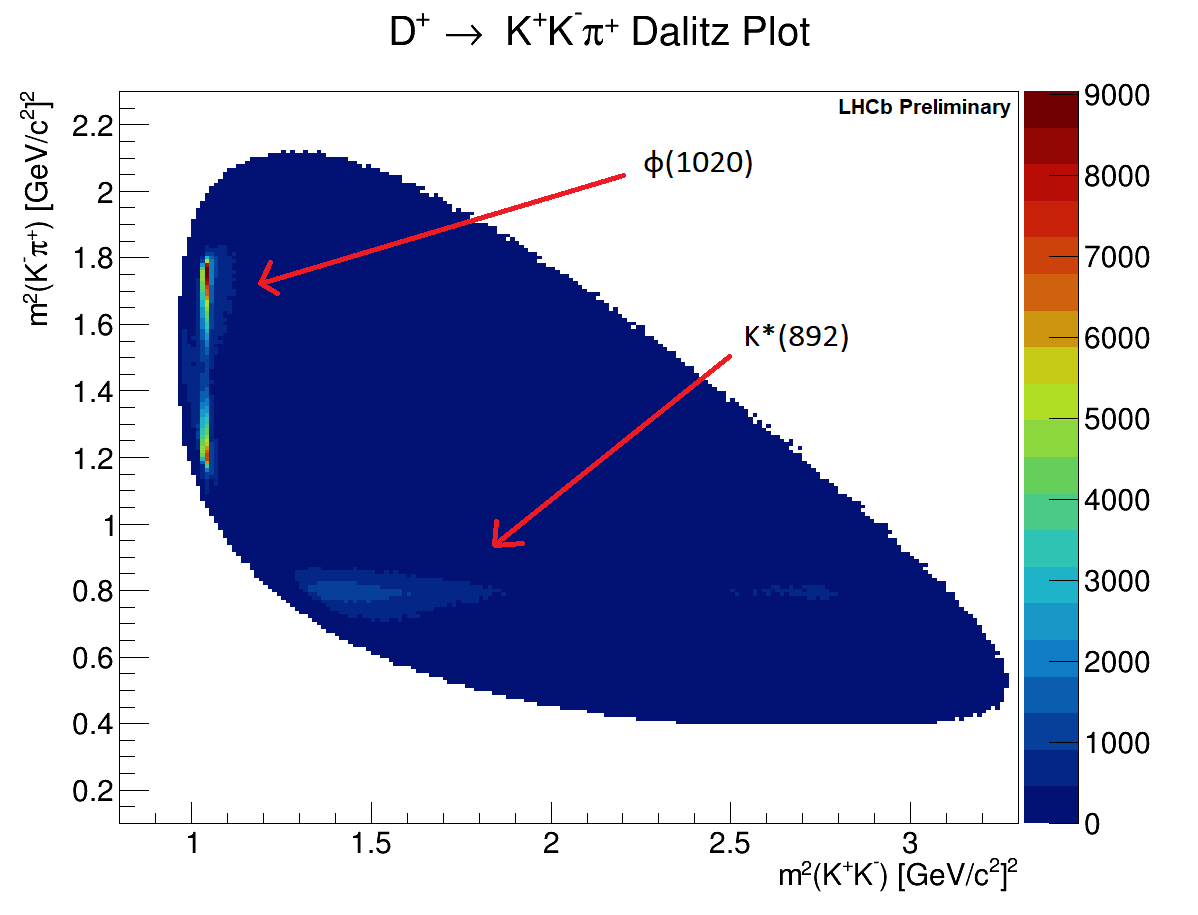
\includegraphics[width=1\linewidth]{dalitz.png}\
  %\label{fig:fringe1}
\end{subfigure}%
\begin{subfigure}{.5\textwidth}
  \centering
  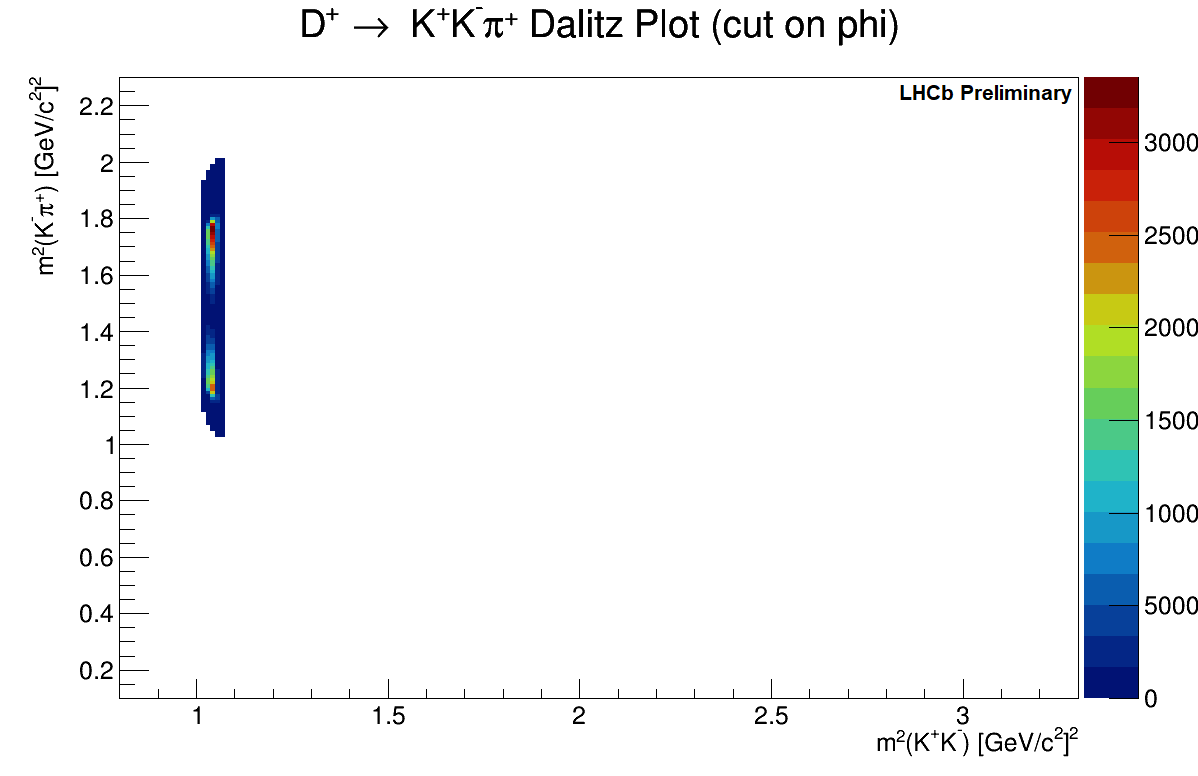
\includegraphics[width=1\linewidth]{dalitzcut.png}
  %\label{fig:fringe2}
\end{subfigure}
\caption{Dalitz plot of $D^{+} \rightarrow K^{+}K^{-}\pi^{+}$ decay before and after the $\phi$ cut.}
\label{fig:dalitz}
\end{figure}


There are a handful of cuts on the reconstructed $D^+_s$ mother particle. The impact parameter $\chi^2$, which is an indicator of the particle's distance of closest approach to the $pp$ interaction vertex is restricted to be less than 4. The flight distance $\chi^2$ is restricted to be greater than 225. This is to ensure a good fit for flight distance to the primary vertex of the decay. The end vertex $\chi^2$, a measure of the agreement between there constructed tracks of final decay particles at their decay vertex, is restricted to be less than 9. Finally, the cosine of the direction angle (DIRA) is restricted to be greater than 0.99999, to ensure that the particle is following closely to the beam.


There is one final part of the selection process that is unique to this analysis and comes from the fact that the $D^+$ data and $D^+_s$ data are stored separately. Ideally, we will have one spectrum of data spanning both the central value of the $D^+$ mass peak and the $D^+_s$ mass peak such that we can have one fit for both peaks simultaneously. However, the raw data for $D^+$ decays spans a reconstructed mass range of $1790 - 1950$ MeV, while the raw data for $D^+_s$ decays spans a range of $1890-2050$ MeV. This leaves us with an "overlap" region in the range of $1890 - 1950$ MeV. For reasons that are not entirely clear, the counts in these bins are \textit{not} equal as one would expect. Figure \ref{fig:overlap} illuminates the issue we face. After cuts the central overlap region bin differences are on the order of $10^0$ whereas the bins themselves are on the order of $10^3$. Since this is relatively small, we choose the center, $1920$ MeV, as the point at which we stop using $D^+$ data and start using $D^+_s$ data to construct a complete spectrum.


\begin{figure}[h!]
\centering
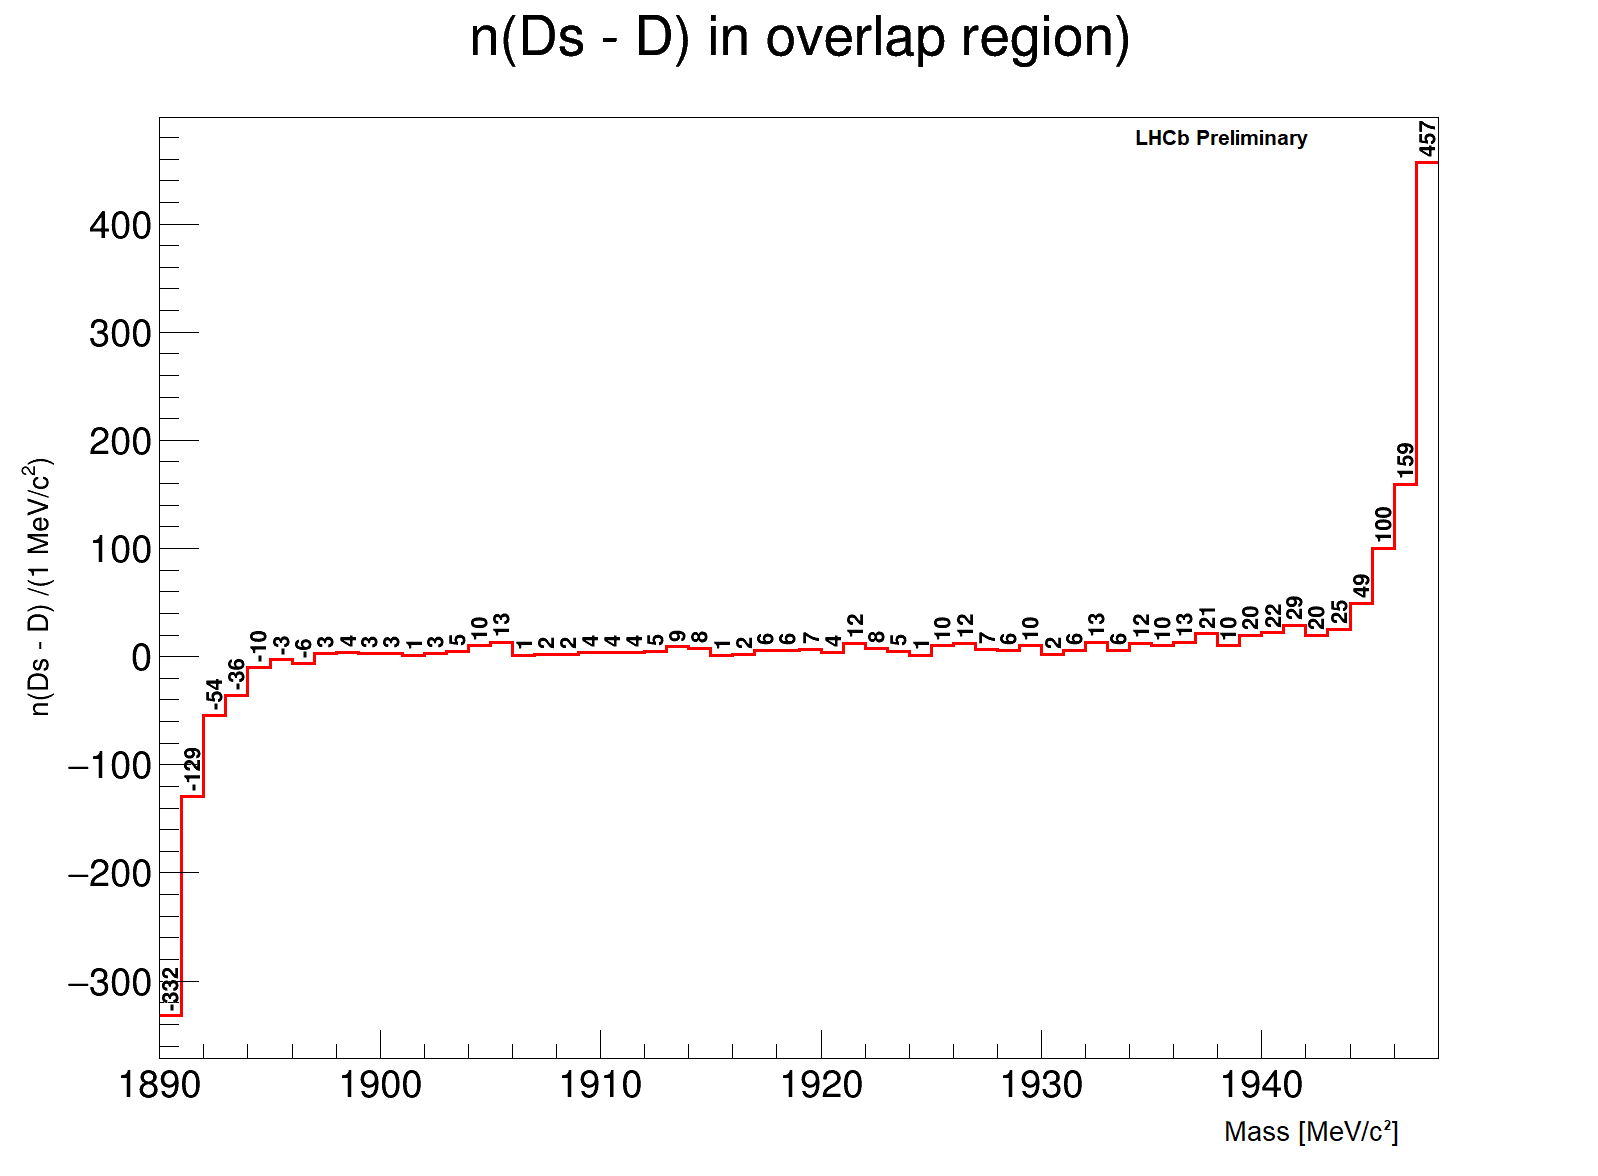
\includegraphics[width=0.6\linewidth]{overlap.png}
\caption{Difference of events in each data set in the overlap region.}
\label{fig:overlap}
\end{figure}







\section{Fit Results}
After all cuts are made and extraneous variables are removed from the data set, we are left with 320 MB of data. This is approximately $0.025\%$ of the original, raw data. The fit is built from six components. The $D^+$ signal is modeled by a Gaussian and a Crystal Ball function with common mean. The $D^+_s$ signal is modeled by a double Gaussian and a Crystal Ball function, all with common mean. The second Gaussian in the $D^+_s$ fit allows for some added flexibility. Crystal Ball functions are composed of a Gaussian core with a power law tail on the lower end. Though they take various forms, an example can be seen in Equation \ref{eqn:CB} where $N$ is a normalization constant. The two Crystal Ball functions for this fit are fixed to have the same parameters, $\alpha$ and $n$. 

\begin{equation}
f(x; \alpha, n, \bar{x}, \sigma) = N \cdot
\begin{cases} 
      \text{exp}(-\frac{(x-\bar{x})^2}{2\sigma^2} & \frac{x - \bar{x}}{\sigma} > -\alpha \\
      (\frac{N}{|\alpha|})^n \cdot \text{exp}(-\frac{|\alpha|^2}{2}) \cdot (\frac{N}{|\alpha|} - |\alpha| - \frac{x - \bar{x}}{\sigma})^{-n}  & \frac{x - \bar{x}}{\sigma} \leq -\alpha \\
   \end{cases}
\label{eqn:CB}
\end{equation}

The "pull plot" is a useful tool when measuring how good a fit is. It is defined in the following way:

\begin{equation}
\text{pull} = \frac{binVal - fitVal}{\sqrt{fitVal}}
\label{eqn:pull}
\end{equation}

where $binVal$ is the real value of a bin and $fitVal$ is the fitted value. When looking at a pull plot, we generally aim for all pulls to be within $5 \sigma$ of the origin. We also hope to see the pulls relatively randomly distributed, indicating that there are no underlying patterns that may have been missed or that the minimization of the fit was poor). 

The final fit can be seen in Figure \ref{fig:fit}. Overall, the fit is pretty good. The pull values are slightly higher than desired in the overlap region, but this is okay considering the bins in this region are on the order of $10^3$ events, whereas bins in the signal regions are on the order of $10^5$ events. There is some periodic motion of the pull throughout the $D^+_s$ signal peak which is likely a result of poor fitting parameters or minimization. The second Gaussian in this peak was implemented to help resolve these issues, and it does a fair amount, but the fit could certainly be better in this area. The uncertainties on all parameters in the fit are small compared to the parameters themselves, which is another indicator of a good fit. The signal-to-background ration on the fit is about 400.



\begin{figure}[h!]
\centering
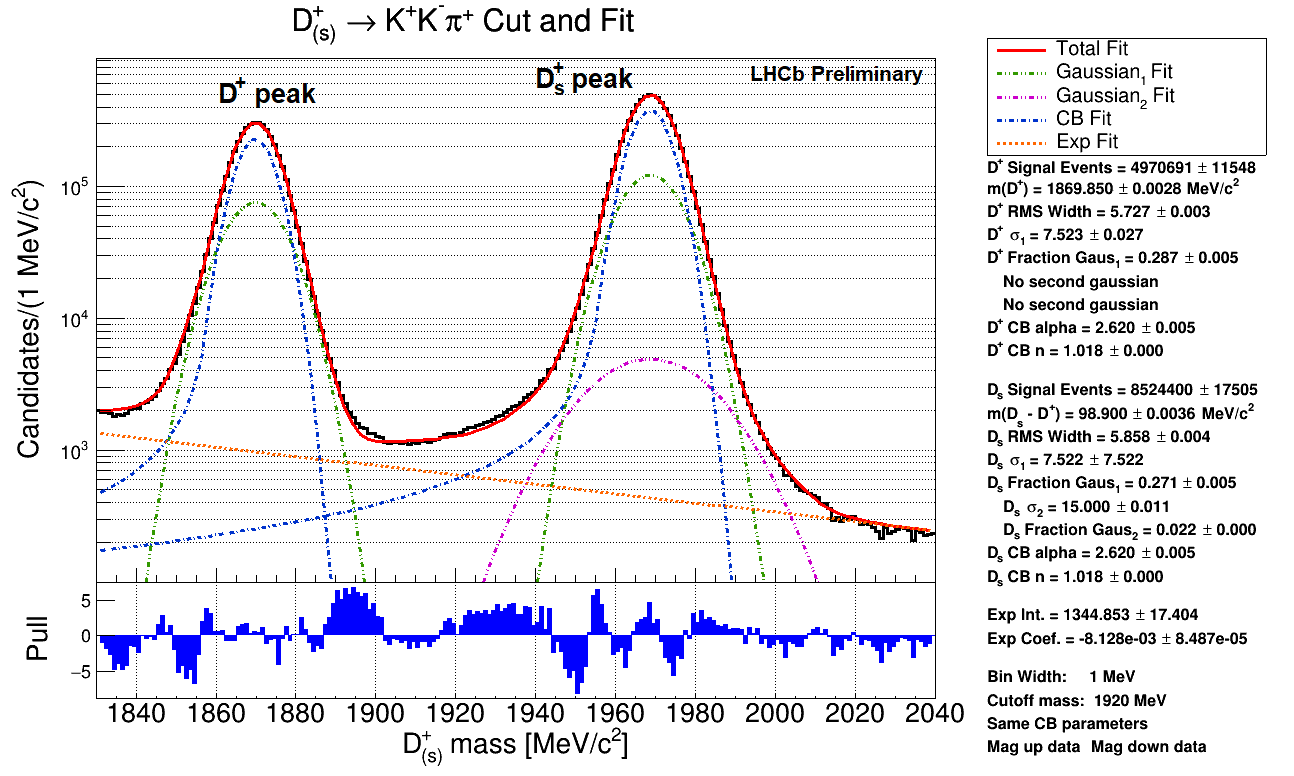
\includegraphics[width=0.9\linewidth]{bigfit.png}
\caption{$D^+$ and $D^+_s$ signal and background fit after all applied cuts.}
\label{fig:fit}
\end{figure}


The fit is repeated twice: once where the mass of the $D^+$ and $D^+_s$ are fit, and a second time where the mass of the $D^+$ is fit and the mass difference $m(D^+_s) - m(D^+)$ is fit. We fit $4,970,691 \pm 11,548$ $D^+$ signal events and $8,524,400 \pm 17,505$ $D^+_s$ signal events. We arrive at the following mass and mass difference measurements:

\begin{center}
$m(D^+) = 1869.850 \pm 0.0029\text{(stat)} \pm x.xxx\text{(syst)}$ MeV/$c^2$\\
$m(D^+_s) = 1968.750 \pm 0.0023\text{(stat)} \pm x.xxx\text{(syst)}$ MeV/$c^2$\\
$m(D^+_s) - m(D^+) = 98.900 \pm 0.0036\text{(stat)} \pm x.xxx\text{(syst)}$ MeV/$c^2$\\
\end{center}




\section{Summary}
As stated before, this is not the first time this measurement has been made via $pp$ collision data- it is simply an attempt to reach a higher precision than it's predecessors. Table 1 and Figure \ref{fig:compare} lay out the development of this measurement over the past 20 years. Table 1 also includes the measurement made at the end of my summer 2020 research term. The improvement in results from then to now is realized by reducing the statistical error by about a factor of 30. From the LHCb measurement in 2013, we have reduced the statistical error by a factor of about 8. As it stands, this measurement is $4\sigma$ away from the PDG average. This is, for now, an admissible deviation. There is still some work do be done on the measurement, especially with regards to the systematics. We believe that such considerations will reduce our measurement, as indicated by the green arrow in Figure \ref{fig:compare}.


\begin{table}
\begin{center}
\begin{tabular}{l | c | c | c | c}
Organization &  Year & $m_{D^+_s} - m_{D^+}$ [MeV] &  $D^+$ Signal Events & $D^+_s$ Signal Events\\
\hline \hline
BaBar\cite{babar} & 2002 & $98.4 \pm 0.3\text{(stat)}$ & $ - $ & $47,794 \pm 311$\\ 
LHCb\cite{lhcb} & 2013 & $98.68 \pm 0.03\text{(stat)}$ & $68,787 \pm 321$ & $248,694 \pm 540$\\
LHCb - UC & 2020 & $98.97 \pm 0.1\text{(stat)}$ & $73,644 \pm 285$ & $12,529 \pm 1602$\\ 
LHCb - UC & 2021 & $98.89 \pm 0.0036\text{(stat)}$ & $4,970,691 \pm 11,548$ & $8,524,400 \pm 17,505$\\ 
\end{tabular}
\label{tab:meas}
\end{center}
\caption{Table of previous $m_{D^+_s} - m_{D^+}$ measurements.}
\end{table}

\begin{figure}[h!]
\centering
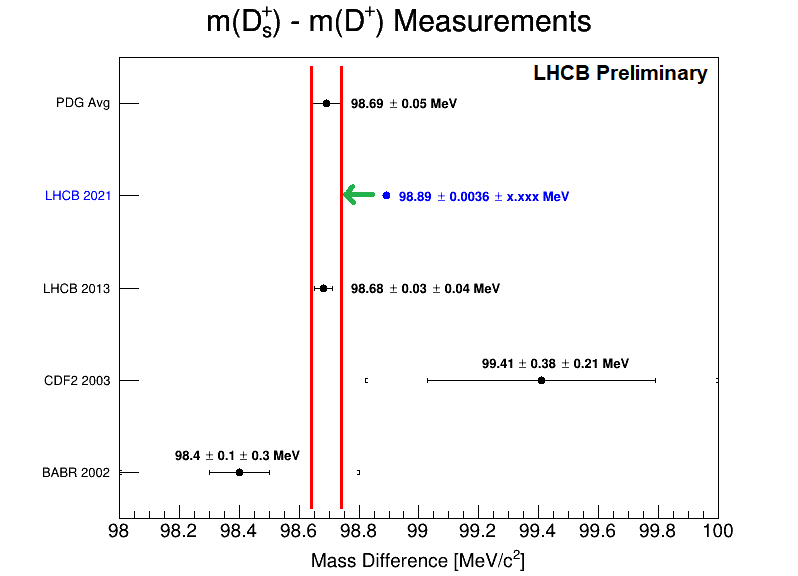
\includegraphics[width=0.7\linewidth]{dp_mass_comparison.png}
\caption{Comparison of $m_{D^+_s} - m_{D^+}$ measurements.}
\label{fig:compare}
\end{figure}




\subsection{Future Work}
As has been alluded to, this measurement has some work to be done before it can be complete. The main focus moving forward will be to establish the systematics of the decay and how to appropriately account for them in the analysis. We believe that the most dominating systematic uncertainty will come from the calibration of the momentum scale of the detector. This issue arises from uncertainties involving the strength of the magnetic field produced by the detector. There are also other systematics to consider, but as for now it is estimated that they will pale in comparison to the momentum scale uncertainty. We estimate the systematic error to be on the same order as the statistical error, or about $3$ keV.




\begin{figure}[h!]
\centering
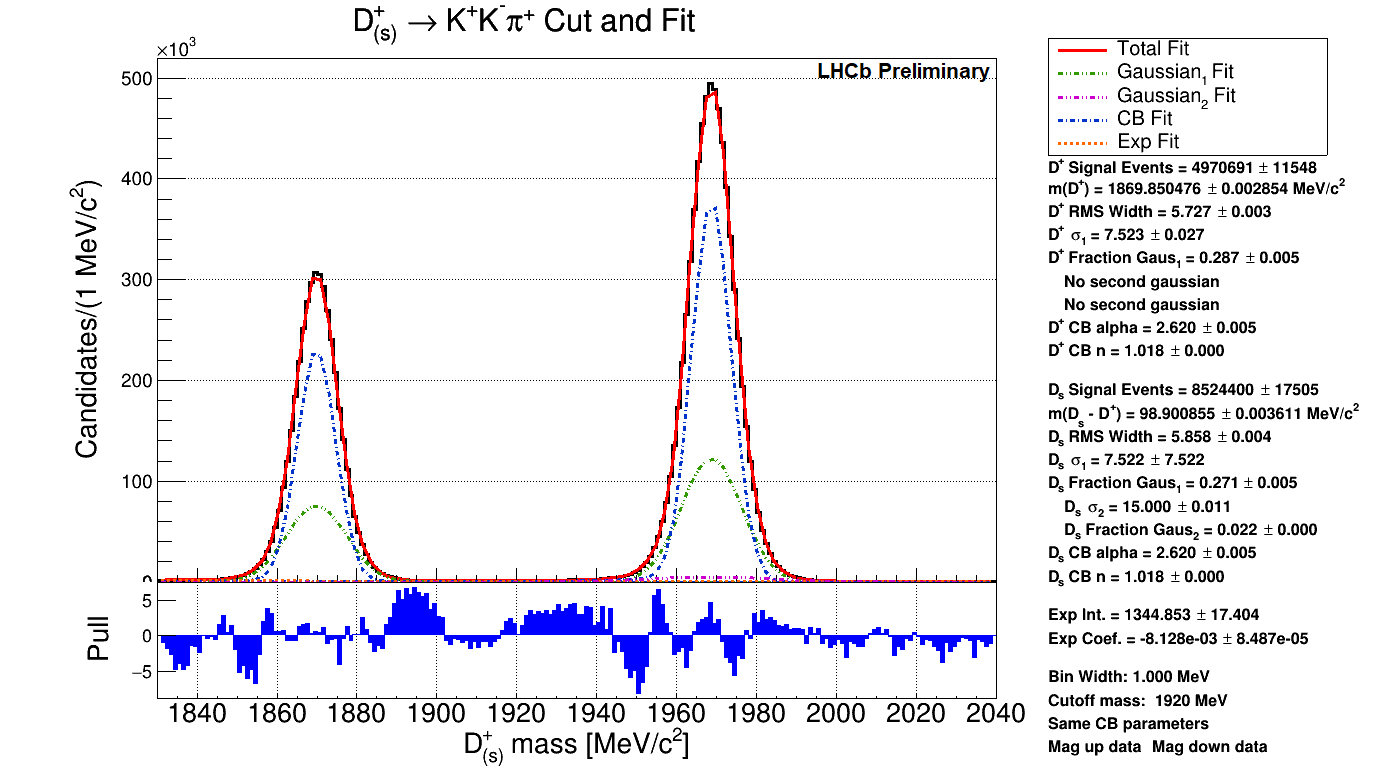
\includegraphics[width=0.8\linewidth]{bigfitlinear.png}
\caption{$D^+$ and $D^+_s$ signal and background fit after all applied cuts (linear y-axis).}
\label{fig:fitlinear}
\end{figure}





\section*{Acknowledgments}
I would like to thank Dr. Michael Sokoloff for helping me through this research. Over the past year I have learned so much, not only abut high energy physics, but about the research process as a whole. His guidance and wisdom have proved invaluable to my advancement as a researcher. I would also like to thank the other students researching under Dr. Sokoloff. To those who had already been a part of the group when I joined and were able to answer so many questions and to those who joined along with myself and helped with the learning process. 
\\
\\
This research was made possible thanks to grants from the National Science Foundation.















\newpage
\newpage

\begin{thebibliography}{9}

\bibitem{theory}
Jose L. Goity, Chandana P. Jayalath,
\textit{Strong and Electromagnetic Mass Splittings in Heavy Mesons},
\texttt{arXiv:hep-ph/0701245}

\bibitem{lhcb} 
LHCb Collaboration, R. Aaij \textit{et al.},
\textit{Precision measurement of D meson mass differences},
\texttt{arXiv:hep-ex/1304.6865}

\bibitem{babar} 
BaBar Collaboration, B. Aubert \textit{et al.},
\textit{Measurement of $D^+_s$ and $D^{*+}_s$ production in B meson decays and from continuum $e^+e^-$ annihilation at $\sqrt{s} = 10.6$ GeV},
Phys. Rev. \textbf{D65} (2002) 091104, \texttt{arXiv:hep-ex/0201041}

\bibitem{pdg}
2020 Review of Particle Physics.
P.A. Zyla et al. (Particle Data Group), Prog. Theor. Exp. Phys. \textbf{2020}, 083C01 (2020)

\bibitem{cerncomp}
CERN. (2018, June). Key Facts and Figures – CERN Data Centre.

\bibitem{detector}
CERN. (2008b). LHCb - Large Hadron Collider beauty experiment. LHCb Public. https://lhcb-public.web.cern.ch/en/detector/detector-en.html

\bibitem{detector2}
CERN. (2021). LHCb. https://home.cern/science/experiments/lhcb\#:\%7E:text=It\%20is\%2021\%20metres\%20long,of\%20Ferney\%2DVoltaire\%2C\%20France.

\bibitem{events}
CERN. (2008). LHCb - Large Hadron Collider beauty experiment. LHCb Public. https://lhcb-public.web.cern.ch/en/Data\%20Collection/Triggers-en.html\#:\%7E:text=When\%20LHCb\%20is\%20up\%20and,million\%20proton\%20collisions\%20every\%20second.

\bibitem{kinematics}
J. Beringer et al. (Particle Data Group), Phys. Rev. D \textbf{86}, 010001 (2012).

\bibitem{QCD}
Fritzsch, H. (2012, September 27). The history of QCD. CERN Courier. https://cerncourier.com/a/the-history-of-qcd/





\end{thebibliography}



\end{document}